 % The main file for CAMP reports
 % Don't put any content in here. 
 % Don't even include content files by using \input or \inlcude. 
 % Put your content to TEXT.TEX or include it there using \input.
 % Uses:
 %		SETTINGS.TEX	contains the settings for this document
 %		COMMANDS.TEX	contains commands which can be used while writing
 %		INFO.TEX			contains the author, title and so on for the cover
 %		COVER.TEX			formats the front cover of the document
 %		ABSTRACT.TEX	contains the abstract to be included (if needed)
 %		TEXT.TEX			contains the actual content of the document
 %		BIB.BIB				containt the BibTeX entries for the document
  
\documentclass[12pt,a4paper,bibtotoc,idxtotoc,headsepline,footsepline,footexclude,BCOR12mm,DIV13]{scrbook}

\usepackage{listings}
\usepackage{url}
\usepackage{algorithm}
\usepackage{color}

\definecolor{Gray}{gray}{0.96}

%%Settings for Java listings
\lstset{%
	language=Java,
	showstringspaces=false,
	basicstyle=\small,
	keywordstyle=\color{blue},
	breaklines=true,
	frame=single,
	commentstyle=\color{green},
	stringstyle=\color{red},
	backgroundcolor=\color{Gray},
	numbers=left,
	xleftmargin=15pt,
	xrightmargin=15pt,
	tabsize=2,
	captionpos=b
}

% include title and author information for the cover
% Set here the title, authors and other stuff to be used for the cover
% This file is used by MAIN.TEX

% set title, authors and stuff for the cover
\def\doctype{Bachelor's Thesis in Information Systems}
\def\title{Guideline for combining and differentiating between CMMN, DMN and BPMN: An indicator-based use case study}
\def\titleGer{Richtlinie zur Kombination und Differenzierung zwischen CMMN, DMN und BPMN: Eine indikatorbasierte Falluntersuchung}
\def\author{Dominik Gerbershagen}
\def\date{November 15, 2016}

% text to appear in the footer
\def\footertext{}
% include settings
% Included by MAIN.TEX
% Defines the settings for the CAMP report document

\renewcommand{\sectfont}{\normalfont \bfseries}        % Schriftart der Kopfzeile

% manipulate footer
\usepackage{scrpage2}
\pagestyle{scrheadings}
\ifoot[\footertext]{\footertext} % \footertext set in INFO.TEX
%\setkomafont{pagehead}{\normalfont\rmfamily}
\setkomafont{pagenumber}{\normalfont\rmfamily}

%% allow sophisticated control structures
\usepackage{ifthen}

% use Palatino as default font
\usepackage{palatino}

% enable special PostScript fonts
\usepackage{pifont}

% make thumbnails
\usepackage{thumbpdf}

%to use the subfigures
\usepackage{subfigure}


\usepackage{colortbl}


%% show program code\ldots
%\usepackage{verbatim}
%\usepackage{program}

%% enable TUM symbols on title page
\usepackage{styles/tumlogo}


\usepackage{multirow}

%% use colors
\usepackage{color}

%% make fancy math
\usepackage{amsmath}
\usepackage{amsfonts}
\usepackage{amssymb}
\usepackage{textcomp}
%\usepackage{yhmath} % für die adots 
%% mark text as preliminary
%\usepackage[draft,german,scrtime]{prelim2e}

%% create an index
\usepackage{makeidx}

% for the program environment
\usepackage{float}

%% load german babel package for german abstract
%\usepackage[german,american]{babel}
\usepackage[german,english]{babel}
\selectlanguage{english}

% use german characters as well
\usepackage[latin1]{inputenc}       % allow Latin1 characters

% use initals dropped caps - doesn't work with PDF
% \usepackage{dropping}

% to cite websites
%\usepackage{biblatex}


\usepackage{styles/shortoverview}
%----------------------------------------------------
%      Graphics and Hyperlinks
%----------------------------------------------------

%% check for pdfTeX
\ifx\pdftexversion\undefined
 %% use PostScript graphics
 \usepackage[dvips]{graphicx}
 \DeclareGraphicsExtensions{.eps,.epsi}
 \graphicspath{{figures/}{figures/review}} 
 %% allow rotations
 \usepackage{rotating}
 %% mark pages as draft copies
 %\usepackage[english,all,light]{draftcopy}
 %% use hypertex version of hyperref
 \usepackage[hypertex,hyperindex=false,colorlinks=false]{hyperref}
\else %% reduce output size \pdfcompresslevel=9
 %% declare pdfinfo
 %\pdfinfo { 
 %  /Title (my title) 
 %  /Creator (pdfLaTeX) 
 %  /Author (my name) 
 %  /Subject (my subject	) 
 %  /Keywords (my keywords)
 %}
 %% use pdf or jpg graphics
 \usepackage[pdftex]{graphicx}
 \DeclareGraphicsExtensions{.jpg,.JPG,.png,.pdf,.eps}
 \graphicspath{{figures/}} 
 
 %% Load float package, for enabling floating extensions
 \usepackage{float}
 
 %% allow rotations
 \usepackage{rotating}
 %% use pdftex version of hyperref
 \usepackage[pdftex,colorlinks=true,linkcolor=black,citecolor=black,%
 anchorcolor=red,urlcolor=black,bookmarks=true,%
 bookmarksopen=true,bookmarksopenlevel=0,plainpages=false%
 bookmarksnumbered=true,hyperindex=false,pdfstartview=%
 ]{hyperref}
%
%\usepackage[pdftex,colorlinks=false,linkcolor=red,citecolor=red,%
% anchorcolor=red,urlcolor=red,bookmarks=true,%
% bookmarksopen=true,bookmarksopenlevel=0,plainpages=false%
% bookmarksnumbered=true,hyperindex=false,pdfstartview=%
% ]{hyperref}
\fi




%% Fancy chapters
%\usepackage[Lenny]{fncychap}
%\usepackage[Glenn]{fncychap}
%\usepackage[Bjarne]{fncychap}

%\usepackage[avantgarde]{quotchap}

% set the bibliography style
%\bibliographystyle{styles/bauermaNum}
%\bibliographystyle{alpha}
\bibliographystyle{unsrt} %apalike
%\bibliographystyle{alphaurl}
%\bibliographystyle{apalike}

% Excel2LaTeX
\usepackage{booktabs, multicol, multirow}

% code
\usepackage{listings}
\lstset{language=Java,captionpos=b,tabsize=3,frame=lines,keywordstyle=\color{blue},commentstyle=\color{darkgreen},stringstyle=\color{red},numbers=left,numberstyle=\tiny,numbersep=5pt,breaklines=true,showstringspaces=false,basicstyle=\footnotesize,emph={label}}
\lstset{basicstyle=\ttfamily\fontsize{5cm}{1em},breaklines=true}
\lstdefinestyle{nonumbers}
{numbers=none, frame=none, keepspaces=true, keywords={}}
\lstdefinestyle{nonumbers2}
{numbers=none, frame=none, keepspaces=true, keywords={}, 
stringstyle=\color{black}}

%\usepackage[algo2e]{algorithm2e}
\usepackage{algorithm}
\usepackage{algorithmicx,algpseudocode}
\usepackage{varwidth}

\usepackage[toc,page]{appendix}

\usepackage[]{hyperref}
\hypersetup{
    pdftitle={\title},
    pdfauthor={\author},
    pdfsubject={Bachelor's Thesis},
    pdfkeywords={BPMN, DMN, CMN, Use case study},
    bookmarksnumbered=false,     
    bookmarksopen=false,         
    bookmarksopenlevel=1,       
    colorlinks=true,            
    pdfstartview=Fit,           
    pdfpagemode=UseOutlines,    % this is the option you were lookin for
    pdfpagelayout=TwoPageRight
}

%acronympage at the beginning 
\usepackage[nohyperlinks]{acronym}

%this package is used to make annotations in latex indicating todo notes or missing figures 
\usepackage{todonotes}

%this package is used for wrapping text around figer 
\usepackage{wrapfig}
% include commands
% Commands to be used within the TUM report document
% Included by MAIN.TEX
% Please include your own cool commands here. 
% Be only sure to comment it sufficiently so others can use it.

%-------------------------------------------------------------
%                      Own Commands
%-------------------------------------------------------------


%-------------------------------------------------------------
% math stuff -------------------------------------------------

% nice R, N, C
\newcommand{\nat}{\mathbb{N}}
\newcommand{\real}{\mathbb{R}}
\newcommand{\compl}{\mathbb{C}}



% norm
\newcommand{\norm}[1]{\left\| #1 \right\|}

% un demi
\newcommand{\half}{\frac{1}{2}}

% parantheses
\newcommand{\parenth}[1]{ \left( #1 \right) }
\newcommand{\bracket}[1]{ \left[ #1 \right] }
\newcommand{\accolade}[1]{ \left\{ #1 \right\} }
%\newcommand{\angle}[1]{ \left\langle  #1 \right\rangle }

% partial derivative: %#1 function, #2 which variable
% simple / single line version
\newcommand{\pardevS}[2]{ \delta_{#1} f(#2) }
% fraction version
\newcommand{\pardevF}[2]{ \frac{\partial #1}{\partial #2} }

% render vectors: 3 and 4 dimensional
\newcommand{\veciii}[3]{\left[ \begin{array}[h]{c} #1 \\ #2 \\ #3	\end{array} \right]}
\newcommand{\veciv}[4]{\left[ \begin{array}[h]{c} #1 \\ #2 \\ #3 \\ #4	\end{array} \right]}

% render matrices: 3  dimensional (arguments in row first order)
\newcommand{\matiii}[9]{\left[ \begin{array}[h]{ccc} #1 & #2 & #3 \\ #4 & #5 & #6 \\ #7 & #8 & #9	\end{array} \right]}
%DOESN'T WORK,DON'T KNOW WHY \newcommand{\mativ}[16]{\left[ \begin{array}[h]{cccc} #1 & #2 & #3 & #4 \\ #5 & #6 & #7 & #8 \\ #9 & #10 & #11 & #12 \\ #13 & #14 & #15 & #16 \end{array} \right]}


%-------------------------------------------------------------
%-------------------------------------------------------------


%-------------------------------------------------------------
% some abreviations ------------------------------------------
\newcommand{\Reg}{$^{\textregistered}$}
\newcommand{\reg}{$^{\textregistered}$ }
\newcommand{\Tm}{\texttrademark}
\newcommand{\tm}{\texttrademark~}
\newcommand {\bsl} {$\backslash$}

%-------------------------------------------------------------
%-------------------------------------------------------------


%-------------------------------------------------------------
% formating --------------------------------------------------

% Theorem & Co environments and counters
\newtheorem{theorem}{Theorem}[chapter]
\newtheorem{lemma}[theorem]{Lemma}
\newtheorem{corollary}[theorem]{Corollary}
\newtheorem{remark}[theorem]{Remark}
\newtheorem{definition}[theorem]{Definition}
\newtheorem{equat}[theorem]{Equation}
\newtheorem{example}[theorem]{Example}
%\newtheorem{algorithm}[theorem]{Algorithm}

% inserting figures
\newcommand{\insertfigure}[4]{ % Filename, Caption, Label, Width percent of textwidth
	\begin{figure}[htbp]
		\begin{center}
			\includegraphics[width=#4\textwidth]{#1}
		\end{center}
		\vspace{-0.4cm}
		\caption{#2}
		\label{#3}
	\end{figure}
}




% referecing figures

\newcommand{\refFigure}[1]{ %label
	figure \ref{#1}
}
\newcommand{\refChapter}[1]{ %label
	chapter \ref{#1}
}

\newcommand{\refSection}[1]{ %label
	section \ref{#1}
}

\newcommand{\refParagraph}[1]{ %label
	paragraph \ref{#1}
}

\newcommand{\refEquation}[1]{ %label
	equation \ref{#1}
}

\newcommand{\refTable}[1]{ %label
	table \ref{#1}
}




\newcommand{\rigidTransform}[2]
{
	${}^{#2}\!\mathbf{H}_{#1}$
}

%code, in typewriter
\newcommand{\code}[1]
 {\texttt{#1}}

% comment that appears on the border - very practical !!!
\newcommand{\comment}[1]{\marginpar{\raggedright \noindent \footnotesize {\sl #1} }}

% page clearing
\newcommand{\clearemptydoublepage}{%
  \ifthenelse{\boolean{@twoside}}{\newpage{\pagestyle{empty}\cleardoublepage}}%
  {\clearpage}}


%-------------------------------------------------------------
%-------------------------------------------------------------


\newcommand{\etAl}{\emph{et al.}\mbox{ }}


% Stoimenov custom commands
%\newcommand{\Pubsub}{Publish/subscribe}
\newcommand{\pubsub}{Publish-Subscribe}
%\newcommand{\PubSub}{Publish/Subscribe}


%\makeindex
\linespread{1.15}

\makeglossary

\begin{document}

	\frontmatter
	
	% The front cover for the TUM report document.
% Included by MAIN.TEX


%--------------------------------------------------
% The Front Cover
%--------------------------------------------------

% The front cover for the TUM document.
% Included by MAIN.TEX


%--------------------------------------------------
% The Front Cover
%--------------------------------------------------

% correct BCOR - undo at the end !!!
\def\bcorcor{0.15cm}
\addtolength{\hoffset}{\bcorcor}

\thispagestyle{empty}

 \vspace{4cm}
\begin{center}
	       \oTUM{4cm}
	   
	   \vspace{5mm}     
	   \huge FAKULT{\"A}T F{\"U}R INFORMATIK\\ 
	   \vspace{0.5cm}
	 \large DER TECHNISCHEN UNIVERSIT{\"A}T M{\"U}NCHEN\\
    \vspace{1mm}
        
	\end{center}
		

\vspace{15mm}
\begin{center}

   {\Large \doctype}

  \vspace{20mm}
  
  {\huge\bf \title}\\%[3ex]
  
  
  \vspace{15mm}
  
  
  {\LARGE  \author}
  
  \vspace{10mm}
  
  \begin{figure}[h!]
  \centering
   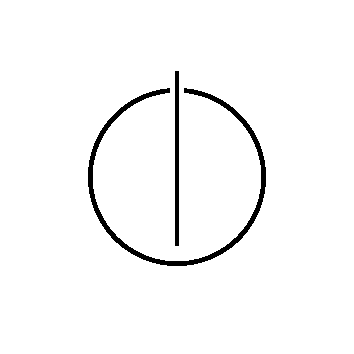
\includegraphics[width=4cm]{styles/informat.png}
  \end{figure}
  
  \end{center}

	\clearemptydoublepage
	
	% The titlepage for the CAMP report document.
% Included by MAIN.TEX


%--------------------------------------------------
% The title page
%--------------------------------------------------

% correct BCOR - undo at the end !!!
\def\bcorcor{0.15cm}
\addtolength{\hoffset}{\bcorcor}

\thispagestyle{empty}

\vspace{10mm}
\begin{center}
	       \oTUM{4cm}
	   
	   \vspace{5mm}     
	   \huge FAKULT{\"A}T F{\"U}R INFORMATIK\\ 
	   \vspace{0.5cm}
	 \large DER TECHNISCHEN UNIVERSIT{\"A}T M{\"U}NCHEN\\        
	 
\end{center}


\vspace{5mm}
\begin{center}

   {\Large \doctype}

  \vspace{5mm}
  
  {\Large \title}\\
  
  
  \vspace{5mm}
  
  
  {\Large  \titleGer}\\
  
  
  \vspace{10mm}

   % \hfill
    \begin{tabular}{ll}
	   \large Author:	& \large \author \\[2mm]
	   \large Supervisor:	& \large Prof. Dr. rer. pol. Hans-Arno Jacobsen  \\[2mm]				
	   \large Advisor:	& \large \begin{minipage}[t]{1.0\columnwidth}
		 Martin Jergler, M.Sc.
	     \end{minipage} \\[10mm]
	     
	   \large Date:	& \large November 15, 2016
	 \end{tabular}
	 
	 \vspace{5mm}
	 
	 \begin{figure}[H]
  \centering
   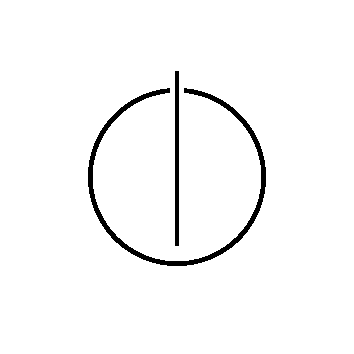
\includegraphics[width=4cm]{styles/informat.png}
  \end{figure}
   

\end{center}

% undo BCOR correction
\addtolength{\hoffset}{\bcorcor}
	
	\clearemptydoublepage


\thispagestyle{empty}
\selectlanguage{german}
	\vspace*{0.6\textheight}
	\noindent
	Ich versichere, dass ich diese Bachelor-Thesis selbst{\"a}ndig verfasst und nur 
	die angegebenen Quellen und Hilfsmittel verwendet habe.
	
	\vspace{20mm}
	
	\selectlanguage{english}
	\noindent
	I confirm that this bachelor's thesis is my own work and I have documented all sources and 		material used.
	
	\vspace{10mm}
	\noindent
	Munich, November 15, 2016 \hspace{4cm} \author
	\selectlanguage{english}
\newpage
	
	% Abstract for the TUM report document
% Included by MAIN.TEX

\clearemptydoublepage
\phantomsection
\addcontentsline{toc}{chapter}{Abstract}	

\vspace*{2cm}
\begin{center}
{\Large \bf Abstract}
\end{center}

	\clearemptydoublepage
	\phantomsection
	\addcontentsline{toc}{chapter}{Table of contents}
	\tableofcontents
  	\clearemptydoublepage
  
	\mainmatter
		\chapter{Introduction}
\label{chapter:introduction}

\section{Motivation}
\label{chapter:motivation}
Since its beginning in the early 1980s, Business Process Management (BPM) has become a large industry and research field. Starting with Business Process Re-engineering (BPR), a radical approach to align internal business processes along the value chain of a company, many subsequent modeling techniques were developed. \\
With the release of Business Process Model and Notation (BPMN) in the early 2000s, a step towards automated process execution has been taken. Since the initial release, BPMN has been examined thoroughly which lead to several positive and negative conclusions. The lack of flexibility for processes that rather require knowledge instead of a strict control flow, only to mention one. For this reason, Case Management Model and Notation (CMMN) was published in 2014. A modeling notation capturing flexible work with focus on knowledge workers and support for run-time adjustment such as planning and skipping tasks, or even adding new ones. \\
Another modeling specification was released in 2015 by the Object Management Group (OMG): the Decision Model and Notation. Where BPMN gets stuck with its vast amount of gateways capturing decisions, DMN becomes relevant by reducing decisions to a single element, the Decision Table. \\
All of the three named modeling techniques contribute to the objective of fully automated process execution and the reduction of routine work. Furthermore, processing data and supporting knowledge-intensive jobs moved to the center of current process modeling and ongoing research. \enlargethispage{1\baselineskip} \newpage

\section{Problem Statement}
\label{chapter:problem_statement}
Business Model and Notation (BPMN) has become a quasi-standard for modeling business processes, logical steps in software-systems or for the alignment of companies along the process chains. BPMN was standardized in 2005 by the Object Management Group (OMG), but had a long list of predecessors including the \textit{Event-driven Process Chain} (EPC), the \textit{Swimlane Visualization}, \textit{Business Process Re-engineering}, to mention only a few. Despite the inheritance of these languages, BPMN is not a fit for all solution. It has positive and negative aspects, which will be discussed in this thesis.\\ 
BPMN works best when it comes to processes that incorporate the \textit{Value Chain Model} by Michael E. Porter \cite{Porter1988}. Every company needs these strict processes to optimize the value chain, for the value creation and to separate the hierarchies between employees and departments. By 2016, however, these processes have been largely automated. For this automation, the BPMN syntax worked very well due to the strict processes that could be automated more or less easily. The next challenge is to implement a process that can help manual workers and deal with data intensive environments. \\
At this point, \textit{Case Management Model and Notation} (CMMN) and \textit{Decision Model and Notation} (DMN) come into play. Both were highly anticipated by people working in modeling departments. This thesis will investigate the benefits of separating the decision logic and case management into these new standards, as well as combining them in a macro model. The weaknesses and strengthens of BPMN, CMMN and DMN will be presented in detail in order to form indicators for when to use which language best. The publication of the two latest standards by the Object Management Group lead to the following research tasks: 

\begin{itemize}
\item Investigation of the new Decision Model and Notation specification published by the Object Management Group, extracting the assets and drawbacks especially concerning the vast modeling of gateways in BPMN. Is DMN the solution to simplify decision-modeling? 
\item Investigation of the Case Management Model and Notation specification by the Object Management Group, particularly how case modeling can be used in a model-driven software development project. 
\item How do CMMN, DMN and BPMN work together in a model-driven software project? Is there a valid possibility to combine all three specifications in one model? Is it possible to improve the process and information flow, readability and eventually implementation of the model by the developer? \enlargethispage{1\baselineskip}  
\end{itemize}

\section{Approach}
\label{chapter:approach}
The intent is to create a guideline for differentiating and combining three modeling languages. The main topics covered are an explanation of the specifications, the main characteristics, a set of tools that identifies each notation and eventually a practical application to show how the guideline works. \\
At first, a background section derived from literature analysis gives an overview of each specification's development up to the recent release of standardization. Followed by a set of process discovery methods derived from a literature review, the reader is instructed on how to aggregate information about processes. Furthermore, the different methodologies are listed with positive and negative aspects, as well as some best practices derived from conference publications. \\
Afterwards, each notation is explained with illustrations, focused on the main characteristics. With the help of the specifications and additional literature, a set of categories and specific terms was constructed aiming at the correct identification of a notation for a given process discovery output. As a consequence, the modeler is able to discover processes and differentiate between the notations. \\
Next, the specifications are examined for technical interfaces to different modeling notations. Along with practical examples, the attributes and references to different notations are shown. Moreover, this part deals with best practices and patterns used to combine different notations. \\
The third chapter is comprised of a practical application to processes taken from the eKultur GmbH. eKultur, as described more detailed in the background chapter, is a software project to digitize the theater production industry. The company has chosen a model-driven development approach with the side effect of generating several process models. After the process discovery phase, the results were used to apply the indicators and check the recommendation system, as well as modeling the processes. A decision-engine was designed to simplify the application of indicators and is presented as well in Chapter \ref{chapter:case_study}. \\
Each model featured in this thesis was created with either \textit{signavio modeler} or \textit{camunda modeler}, relating to either a specific process taken from eKultur GmbH or a certain use case which has an explanation next to it. \newpage

\section{Contributions}
\label{chapter:contributions}
Since the release of CMMN in 2014 and DMN in 2015, recent publications deal with their realization in platforms and the proof of concept, e.g. \cite{KurzSchmidtFleischmannEtAl2015}, \cite{Fish2012}, \cite{OsuszekStanek2015}. Recent publications deal with Case Management or Decision Management on a higher level concept while former publications incorporate a broader research field influencing the notation as well. \\
None of the publications, however, deal with the combination of all three modeling languages or the objective to take process discovery results and examine them for a fitting modeling notation. This thesis contributes to the BPM research field in two ways: as a summary of the current state of these three notations and best practices, as well as a methodology to identify a suitable notation for a given process documentation. 

\section{Organization}
\label{chapter:organization}
Before the actual analysis and creation of the guideline commences in Chapter \ref{chapter:indicators}, Chapter \ref{chapter:background} illustrates the development of the each specification's origins up to the current state. To understand the usage and necessity for each specification, it is important to understand what researchers and people from the corresponding industries motivated to develop a new modeling language. \\
The background part is followed by the compilation of indicators. Each modeling language has a certain domain where it works best. The intent of this thesis is to serve as a guideline to differentiate between and combine the three named modeling languages. As a consequence, the indicators will help analysts with the decision-making process and identify the appropriate modeling language for a given process. \\
In Chapter \ref{chapter:combination}, each specification is examined for interfaces to different modeling techniques, followed by the case study that shows a practical application of the indicators on process models taken from eKultur GmbH. This part also deals with the results found in the case study. \\
In the last chapter, we discuss the indicators and the case study, as well as positive and negative aspects of this thesis. Furthermore, recommendations for future work are provided.
		\chapter{Preliminaries}
\label{chapter:preliminaries}
		\chapter{Example}
\label{Example}

A citatation goes like this~\cite{latex}

\begin{figure}
\centering
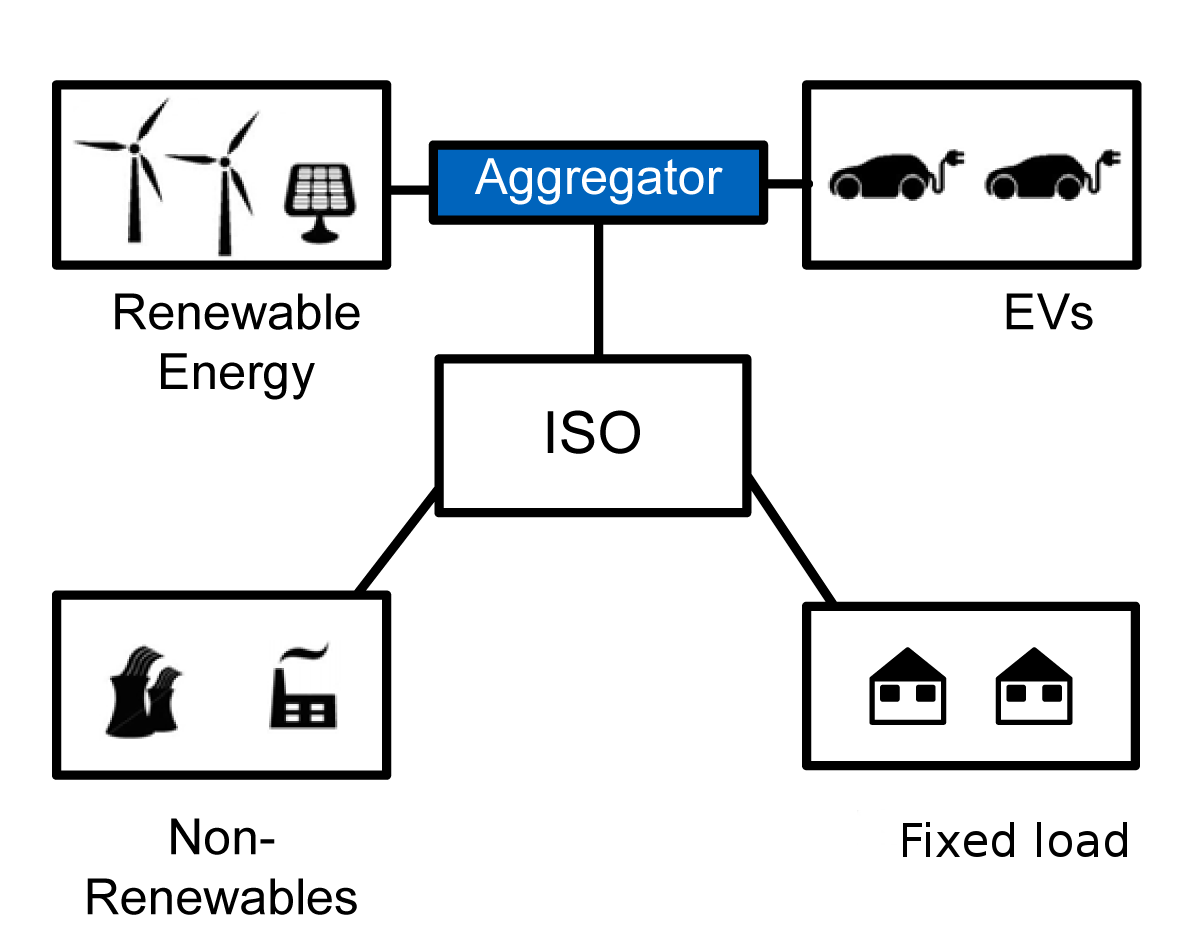
\includegraphics[width=0.8\linewidth]{figures/DirectCoupling}
\caption[Short caption for List of Figures]{Long caption. Displayed below the figure}
\label{fig:DirectCoupling}
\end{figure}

\begin{lstlisting}[language=java, basicstyle=\tiny, frame=single,	stringstyle=\color{red}, backgroundcolor=\color{Gray}, keywordstyle=\color{blue}, stringstyle=\color{red},commentstyle=\color{green},numbers=left, tabsize=2, label=lst:ev, caption={Implementation of Electric Vehicle for OVF.}, breaklines=true, captionpos=b]
public class OVF_EV extends ControllableDevice {
	public static final double EV_THRESHOLD = 0.001;
  private DopsVector value;
  private double requiredEnergy;
  private double[] drivingProfile; 	
  private double lowerChargingBound = 0;
  private double upperChargingBound = 4;

  public void initialize(File file) {
    MatFileReader mfr = new MatFileReader(file);
    MLDouble driveP = (MLDouble) mfr.getMLArray("d"); // driving profile
    drivingProfile = MatrixUtil.getFirstRow(driveP.getArray(), driveP.getN());
    MLDouble requiredE = (MLDouble) mfr.getMLArray("R"); // required energy
    requiredEnergy = requiredE.getArray()[0][0];
    value = new DopsVector(0);
  }

  public DopsVector getValue() {
    return value;
  }	
}
\end{lstlisting}

		
		
		% ---------------------------------------------------------------------------
		%
		% Appendix
		%
		% ---------------------------------------------------------------------------
		%\newpage
%		\part*{Appendix}
%		\addcontentsline{toc}{part}{Appendix}
%		\appendix %---------------------------------------
%		\begin{appendices}
%		\input{chapters/oneAppendix}
%		\end{appendices}
%		\appendix
		\renewcommand\thechapter{}
%		\renewcommand\thesection{\arabic{section}}
		\renewcommand\thesection{}
%		\input{chapters/oneAppendix}

	\clearemptydoublepage		
	\phantomsection
	\addcontentsline{toc}{chapter}{\listfigurename}
	\listoffigures 
	
    \clearemptydoublepage
	\bibliography{bibliography/literature}
	
	
 
\end{document}

